\documentclass[aspectratio=169,10pt]{beamer}

\usepackage{graphicx}
\usepackage{tikz}
\usetikzlibrary{positioning,arrows.meta}
\usepackage{xcolor}
\usepackage{booktabs}
\usepackage{tabularx}
\usepackage{array}
\usepackage{ragged2e}

\definecolor{GEUBlue}{RGB}{20,55,105}
\definecolor{GEULightBlue}{RGB}{238,244,251}
\definecolor{GEUGrey}{RGB}{90,90,90}
\definecolor{GEULightGrey}{RGB}{245,246,248}

\usetheme{default}
\setbeamertemplate{navigation symbols}{}
\setbeamertemplate{blocks}[rounded][shadow=false]
\setbeamersize{text margin left=5mm,text margin right=5mm}
\setbeamercolor{normal text}{fg=black,bg=white}
\setbeamercolor{frametitle}{fg=GEUBlue}
\setbeamercolor{structure}{fg=GEUBlue}
\setbeamercolor{block title}{fg=GEUBlue,bg=GEULightBlue}
\setbeamercolor{block body}{fg=black,bg=GEULightBlue}
\setbeamerfont{frametitle}{size=\large,series=\bfseries}

% Replace with the actual logo filename
\newcommand{\GEULogo}{graphicera_logo.jpeg}

% Header and footer
\setbeamertemplate{headline}{%
  \begin{tikzpicture}[remember picture,overlay]
    \node[anchor=north east,xshift=-0.25cm,yshift=-0.10cm]
      at (current page.north east)
      {\includegraphics[height=0.48cm]{\GEULogo}};
  \end{tikzpicture}
  \vspace{0.48cm}
}
\setbeamertemplate{frametitle}{%
  \vspace{0.01cm}
  \insertframetitle\par
  \vspace{0.02cm}
  \textcolor{GEUBlue}{\rule{\textwidth}{0.9pt}}
  \vspace{0.01cm}
}
\setbeamertemplate{footline}{%
  \leavevmode
  \hbox{%
  \begin{beamercolorbox}[wd=.82\paperwidth,ht=0.20cm,dp=0.05cm,leftskip=.3cm]{author in head/foot}
    \tiny Department of Computer Science \& Engineering | Graphic Era (Deemed to be University)
  \end{beamercolorbox}%
  \begin{beamercolorbox}[wd=.18\paperwidth,ht=0.20cm,dp=0.05cm,rightskip=.3cm]{date in head/foot}
    \hfill\tiny\insertframenumber/\inserttotalframenumber
  \end{beamercolorbox}}
}

\newcommand{\smallnote}[1]{\vspace{0.08cm}{\scriptsize\color{GEUGrey}#1}}
\newcommand{\placeholder}[1]{\textit{\color{GEUGrey}#1}}

\title{\textbf{Project-Based Learning}\\[2mm]\large Phase-I Evaluation}
\author{\textbf{Project Title}\\Team ID: XXXX}
\institute{Department of Computer Science \& Engineering\\Graphic Era (Deemed to be University), Dehradun}
\date{Academic Session 2026--27}

\begin{document}

% 1
\begin{frame}[plain]
\begin{tikzpicture}[remember picture,overlay]
\draw[GEUBlue,line width=3pt] (current page.north west) -- (current page.north east);
\node[anchor=north east,xshift=-0.45cm,yshift=-0.35cm] at (current page.north east)
{\includegraphics[height=1.0cm]{\GEULogo}};
\node[align=center,text width=.84\paperwidth] at ([yshift=.25cm]current page.center)
{{\color{GEUBlue}\fontsize{26}{30}\selectfont\bfseries PROJECT-BASED LEARNING}\\[3mm]
 {\fontsize{18}{22}\selectfont PHASE-I EVALUATION}\\[7mm]
 {\color{GEUGrey}\Large\bfseries ASLConnect: Inclusive Communication}\\[3mm]
 {\color{GEUBlue}\normalsize Team ID: DSCPP-III-2026-T059}};
\node[align=center,anchor=south,yshift=.42cm] at (current page.south)
{\bfseries Department of Computer Science \& Engineering\\
Graphic Era (Deemed to be University), Dehradun\\[-1mm]
\scriptsize Academic Session 2026--27};
\end{tikzpicture}
\end{frame}

% 2
\begin{frame}{Team \& Mentor Details}
\begin{columns}[T,totalwidth=\textwidth]
\column{.48\textwidth}
\begin{block}{Team Information}
\begin{tabular}{@{}ll@{}}
\textbf{Team ID:} & DSCPP-III-2026-T059\\
\textbf{Semester:} & 3rd \\
\textbf{Section:} & A , DS1, ML1\\
\textbf{Domain:} & \placeholder{Computer Science}
\end{tabular}
\end{block}
\column{.48\textwidth}
\begin{block}{Team Members}
1.\quad \placeholder{Srishti Dhasmana -- 2510010598}\\
2.\quad \placeholder{Ishita Bijalwan-- 2510380152}\\
3.\quad \placeholder{Nandini Rana -- 2510370024}\\

\end{block}
\end{columns}
\vspace{1mm}
\begin{block}{Mentor}
\placeholder{Mr.Manish Mehta}
\hfill
\textbf{Interactions completed: 2} 
\end{block}
\end{frame}

% 3
\begin{frame}{Problem Statement \& Motivation}
\begin{block}{Problem Statement}
\placeholder{Individuals with hearing impairments often struggle to be part of everyday conversations, while most hearing people lack any knowledge of sign language. This gap exists largely because sign language is seen as difficult to learn, with few structured resources available. Our project aims to bridge this divide by making ASL easier to learn and understand, fostering more inclusive communication for all.}
\end{block}
\vspace{1mm}
\begin{columns}[T,totalwidth=\textwidth]
\column{.48\textwidth}
\textbf{\color{GEUBlue}Motivation}
\begin{itemize}\itemsep1pt
\item \placeholder{No structured path to learn ASL.}
\item \placeholder{Limits inclusive communication.}
\item \placeholder{No organised data pattern to learn.}
\end{itemize}
\column{.48\textwidth}
\textbf{\color{GEUBlue}Target Users / Stakeholders}
\begin{itemize}\itemsep1pt
\item \placeholder{Family of impaired people.}
\item \placeholder{Educators, and intepretors in training.}
\item \placeholder{Faster, structured learning that improves communication}
\end{itemize}
\end{columns}
\end{frame}

% 4
\begin{frame}{Objectives}
\textbf{\color{GEUBlue}Project Objectives}
\vspace{1mm}
\begin{enumerate}\itemsep1pt
\item \placeholder{Develop a web-based solution to simplify ASL learning.}
\item \placeholder{Implement core features using C++ and DSA concepts.}
\item \placeholder{Apply DSA logic (searching, sorting, data organization) to structure lessons.}
\item \placeholder{Test the system for accuracy and performance.}
\item \placeholder{Demonstrate real-world use and future scope for expansion}
\end{enumerate}
\vfill
\begin{center}
\colorbox{GEULightBlue}{\parbox{.80\textwidth}{\centering
\textbf{Key Objective:} \placeholder{"Enable users to learn and correctly recognize at least the ASL alphabet and basic words through structured lessons, with measurable improvement in sign accuracy and lesson completion rate."}}}
\end{center}
\end{frame}

% 5
\begin{frame}{Proposed Solution}
\begin{columns}[T,totalwidth=\textwidth]
\column{.48\textwidth}
\textbf{\color{GEUBlue}Proposed Approach}
\begin{enumerate}\itemsep1pt
\item \placeholder{Input / Data Collection}
\item \placeholder{Processing / Core Algorithm}
\item \placeholder{System Logic}
\item \placeholder{Database / Storage}
\item \placeholder{Output / Visualization}
\end{enumerate}
\column{.48\textwidth}
\textbf{\color{GEUBlue}Key Features}
\begin{itemize}\itemsep1pt
\item \placeholder{Interactive ASL Lessons}
\item \placeholder{Text to Sign Matching}
\item \placeholder{Gesture Recognition and Validation}
\item \placeholder{Progress Tracking and Scoring}
\item \placeholder{Visual Feedback}
\end{itemize}
\end{columns}
\vfill
\smallnote{An interactive website is designed to teach American Sign Language (ASL) using C++ and DSA concepts. User inputs such as text or gestures are collected and processed through efficient algorithms for recognition and matching. The system logic ensures smooth flow and error handling, while structured data storage using arrays, linked lists, and hash maps enables quick retrieval and scalability. Finally, visual outputs like animations and images provide immediate feedback, making ASL learning engaging, accessible, and efficient while reinforcing computational thinking.}
\end{frame}

% 6
\begin{frame}{Integration of PBL Course Concepts}
\scriptsize
\begin{center}
\renewcommand{\arraystretch}{1.25}
\begin{tabularx}{.96\textwidth}{@{}>{\bfseries}p{3.0cm}X p{2.5cm}@{}}
\toprule

Course & Concepts Applied & Project Module\\
\midrule
Data Structures in C &
\placeholder{Arrays, Linked Lists, Trees, Graphs, Hashing, etc.} &
Lesson Structuring \& Sign Lookup Module\\
OOPs with C++ &
\placeholder{Classes, Inheritance, Polymorphism, STL, etc.} &
Gesture Recognition Engine\\
\midrule
Web Design &
\placeholder{Styling, Navigation, User Interaction, Content} &
Website Frontend (HTML/CSS/JS)\\
\midrule
Computer Vision &
\placeholder{Hand Landmark Detection, Contour Analysis, Real-time Tracking} &
Gesture Recognition Engine\\
\bottomrule
\end{tabularx}
\end{center}
\end{tabularx}
\end{center}
\vfill
\begin{center}
\colorbox{GEULightBlue}{\parbox{.86\textwidth}{\centering
\textbf{Requirement:} Demonstrate meaningful integration of both subjects in \textbf{one} project.}}
\end{center}
\end{frame}

% 7
\begin{frame}{System Architecture / Workflow}
\begin{center}
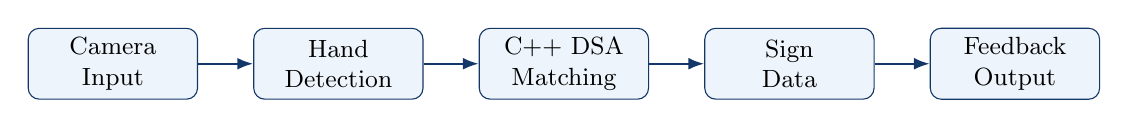
\begin{tikzpicture}[
node distance=7mm,
box/.style={rectangle,rounded corners,draw=GEUBlue,fill=GEULightBlue,
minimum width=2.15cm,minimum height=9mm,align=center,font=\small},
arrow/.style={-{Latex[length=2mm]},thick,draw=GEUBlue}
]
\node[box] (a) {Camera\\Input};
\node[box,right=of a] (b) {Hand\\Detection};
\node[box,right=of b] (c) {C++ DSA\\Matching};
\node[box,right=of c] (d) {Sign\\Data};
\node[box,right=of d] (e) {Feedback\\Output};
\draw[arrow] (a)--(b); \draw[arrow] (b)--(c); \draw[arrow] (c)--(d); \draw[arrow] (d)--(e);
\end{tikzpicture}
\end{center}
\vspace{3mm}
\begin{columns}[T,totalwidth=\textwidth]
\column{.48\textwidth}
\textbf{\color{GEUBlue}Major Components}
\begin{itemize}\itemsep1pt
\item Website Frontend (HTML/CSS/JS)
\item Computer Vision Module (Hand Detection)
\item C++ DSA Engine (Sign Matching)
\end{itemize}
\column{.48\textwidth}
\textbf{\color{GEUBlue}Data / Control Flow}
\begin{itemize}\itemsep1pt
\item User selects lesson $\rightarrow$ website shows sign
\item Webcam captures gesture $\rightarrow$ landmarks extracted
\item C++ engine matches sign, feedback shown to user
\end{itemize}
\end{columns}
\end{frame}

% 8
\begin{frame}{Technology Stack \& Methodology}
\begin{columns}[T,totalwidth=\textwidth]
\column{.48\textwidth}
\begin{block}{Technology Stack}
\begin{itemize}\itemsep1pt
\item Programming: C++, HTML, CSS, JavaScript
\item Data Storage: JSON / Structured Files
\item Tools / Library: OpenCV (Computer Vision)
\item IDE: VS Code
\item Version Control: Git / GitHub
\end{itemize}
\end{block}
\column{.48\textwidth}
\begin{block}{Development Methodology}
\begin{enumerate}\itemsep1pt
\item Problem \& Requirement Analysis
\item Designing Lesson Structure \& DSA Logic
\item Website \& Gesture Engine Implementation
\item Gesture Accuracy Testing
\item Performance \& Usability Evaluation
\end{enumerate}
\end{block}
\end{columns}
\vfill
\begin{center}
\smallnote{Justify the selection of technologies and methodology.}
\end{center}
\end{frame}

% 9
\begin{frame}{Initial Progress \& Team Contribution}
\begin{columns}[T,totalwidth=\textwidth]
\column{.44\textwidth}
\textbf{\color{GEUBlue}Progress Achieved}
\begin{itemize}\itemsep1pt
\item Background / literature study on ASL learning gaps
\item Requirements identified (lesson structure, gesture recognition)
\item System architecture \& workflow designed
\item Website skeleton (HTML/CSS/JS) implemented
\item DSA logic planned for lesson \& sign data structuring
\end{itemize}
\column{.52\textwidth}
\textbf{\color{GEUBlue}Individual Contribution}
\vspace{1mm}
\scriptsize
\begin{tabularx}{\textwidth}{@{}p{1.8cm}p{2.0cm}X@{}}
\toprule
Member & Role & Contribution\\
\midrule
M1 & Lead - Frontend and UI & HTML, CSS, JavaScript Interface\\
M2 & DSA and Backend & C++/DSA Implementation, Data Management\\
M3 & CV/ML Developer & OpenCV, ASL Recognition, Dataset\\

\bottomrule
\end{tabularx}
\end{columns}
\end{frame}

% 10
\begin{frame}{Roadmap, Expected Outcomes \& References}
\begin{columns}[T,totalwidth=\textwidth]
\column{.47\textwidth}
\textbf{\color{GEUBlue}Roadmap}
\begin{enumerate}\itemsep1pt
\item Phase-I: Proposal \& Design
\item Phase-II: Development
\item Phase-III: Final Implementation
\end{enumerate}
\vspace{1mm}
\textbf{\color{GEUBlue}Expected Outcomes}
\begin{itemize}\itemsep1pt
\item Working ASL learning website with structured lessons
\item Functional gesture recognition for basic ASL signs
\item Faster, more accessible ASL learning for beginners
\item Scope to expand vocabulary \& add more sign languages
\end{itemize}
\column{.47\textwidth}
\textbf{\color{GEUBlue}References}
\begin{enumerate}\itemsep1pt
\item ASL Alphabet Dataset -- M (grassknoted/asl-alphabet)
\item MediaPipe Hands -- Google, hand landmark detection framework
\item OpenCV documentation -- opencv.org
\item A. Amin et al., "Open-Source ASL Fingerspell Recognition and Semantic Pose Retrieval Interface," arXiv:2408.09311
\end{enumerate}
\vfill
\begin{center}
\colorbox{GEUBlue}{\parbox{.78\textwidth}{\centering\color{white}\textbf{Thank You}\\Questions \& Suggestions}}
\end{center}
\end{columns}
\end{frame}

\end{document}
